\documentclass{article}
\usepackage{amsmath}
\usepackage{graphicx}
\usepackage{amssymb}

\title{DaBA}
\author{Keith Goh}
\begin{document}
\maketitle
\section{SQL}
\begin{verbatim}
SELECT c1,c2 from t;
\end{verbatim}
Query Data in columns c1 and c3 from table t\\
\begin{verbatim}
SELECT * from t
\end{verbatim}
Query all rows and columns from from table\\
\begin{verbatim}
SELECT c1,c2 from t;
Where condition;
\end{verbatim}
Query data and filter rows with a condition\\
\begin{verbatim}
SELECT c1,c2 from t;
order By c1(DESC/ASC)

SELECT column_name AS alias_name
FROM table_name;
SELECT OrderID, Quantity,
CASE
    WHEN Quantity $>$ 30 THEN "The quantity is greater than 30"
    WHEN Quantity = 30 THEN "The quantity is 30"
    ELSE "The quantity is under 30"
END AS QuantityText
FROM OrderDetails;
\end{verbatim}
(creates 3 columns)
\begin{verbatim}
SELECT IFNULL(NULL, "W3Schools.com");
\end{verbatim}
replace null with W3schools\\
\begin{verbatim}
SELECT Artist.Name,
InvoiceLine.UnitPrice * InvoiceLine.Quantity AS TrackSales
FROM ((InvoiceLine INNER JOIN Track ON
InvoiceLine.TrackId = Track.TrackId )
INNER JOIN Album ON Track.AlbumId = Album.AlbumId)
INNER JOIN Artist ON Album.ArtistId=Artist.ArtistId

Create Table Revenue class as select * from t1
\end{verbatim}
create new table revenue class from t1 all columns
\begin{verbatim}
Delete from track where genreid=20

UPDATE t
SET c1=newvalue
c2=newvalue2
where condition;
updates values in the column c1,c2 that matches the condition.
Select C1,aggregate(c2)
From t
Group By c1
having conditions
\end{verbatim}
Group rows using an aggregate function,eg Count(),Sum(),Avg(),Min().Max()\\
filter groups using having clause\\
The HAVING clause was added to SQL because the WHERE keyword could not be used with aggregate functions.\\
EG.
\begin{verbatim}
SELECT Student, SUM(score) AS total FROM Marks GROUP BY Student
HAVING total > 70
\end{verbatim}

LEFT JOIN: Return all records from the left table, and the
matched records from the right table\\The GROUP BY statement groups rows that have the same values into summary rows, like "find the number of customers in each country".\\
\section{Throughput}
Throughput of a multi-stage process (sometimes called
“Capacity”) is the lowest throughput (rate) among all the stages\\
For Parallel activities,The overall throughput is the minimum throughput among all the parallel activities.\\
Throughput for Multiple Paths,denoted with a diamond when split, find the throughput of slowest. if it is determined that there is a fixed split, if not we assign the calculate add the total rate of the work.\\
\section{R}
the [1] refers to the index of its element\\
rm(input)=remove the input\\
str() is to see the structure of the input\\
c() concatenate function to add variables together to form a vector or vectors together to form a longer one.\\
1:4 works in r to create a list form 1 to 4\\
use arrow function in R\\
\begin{verbatim}
  here <- function(x,y){
    x+y
  }
\end{verbatim}
\begin{verbatim}
  a  <- 1:10/5
  > a
   [1] 0.2 0.4 0.6 0.8 1.0 1.2 1.4 1.6 1.8 2.0

   if ( test_expression1) {
   statement1
   } else if ( test_expression2) {
   statement2
   } else if ( test_expression3) {
   statement3
   } else {
   statement4
   }
\end{verbatim}
default values work\\
\begin{verbatim}
  model <- Taste ~ 0+acetic
  result <- lm(model,ccdata)
\end{verbatim}
use this to declare no constant term\\
\begin{verbatim}
  fit <- result$fitted.values
  taste <- ccdata$Taste
  r1 <- c(0,max(ccdata$Taste$))
  lines(r1,r1)
  title('actual vs. fitted values')
  residuals <- taste-fit
  plot(taste,residuals)
  lines(r1,c(0,0))
  lines(lowess(taste,residuals,f=0.8),col=c('red'))
  title('residuals vs actual values')
\end{verbatim}
AIC the lower the better\\
\begin{verbatim}
admitmodel <- admit ~ gre+gpa
admitresult <- glm(admitmodel,family=binomial,data=graddata)
\end{verbatim}
$$
p=\frac{1}{1+e^{-(-4.949378+0.002691\times gre+0.754687\times gpa)}}
$$
for categorical data we need to use
\begin{verbatim}
  graddata$school_rank <- factor(graddata$school_rank)
\end{verbatim}
for counts/proportion\\
\begin{verbatim}
  ingotdata$frac_not_ready <- ingotdata$Num_Not_ready/ingotdata$Num_ingots
  ingotmodel<-frac_not_ready ~ soak+heat
  #use a generalized linear model in the binomial family

  ingotresult <- glm(ingotmodel,family=binomial,data=ingotdata,weight=Num_ingots)
  summary(ingotresult)

\end{verbatim}
Dependent variable must be a number between 0 and 1\\
we must specify the ni counts which is the weight\\
use AIC to pick best model\\
\begin{verbatim}
setwd ('C:\\Users\\silentfatez\\Downloads')
creditdata <- read.csv("CreditData.csv")
head (creditdata)
plot(creditdata[,c(5,9:14)])
cor(creditdata[,c(5,9:14)])

install.packages("tree")
library(tree)

tree.credit=tree(Status~.,data=creditdata)
summary(tree.credit)
plot(tree.credit)
text(tree.credit,pretty=0)

\end{verbatim}
Top part is for corr data, close to -1 and 1 means its correlated,closer to 0 means its not.\\
Connect R to SQL\\
\begin{verbatim}
  getextract <- function(query){
  dbname <- 'eg.sqlite'
  conn <- dbconnect(SQLITE(),dbname)
  queryresult <- dbGetquery(conn,query)
  dbDisconnect(conn)
  queryresult
  }
  getextract("SELECT FROM NEWEXTRACT Limit 20")
\end{verbatim}
\section{GIS}
GIS rmb longtitude is like length so x then latitude is like high so y\\
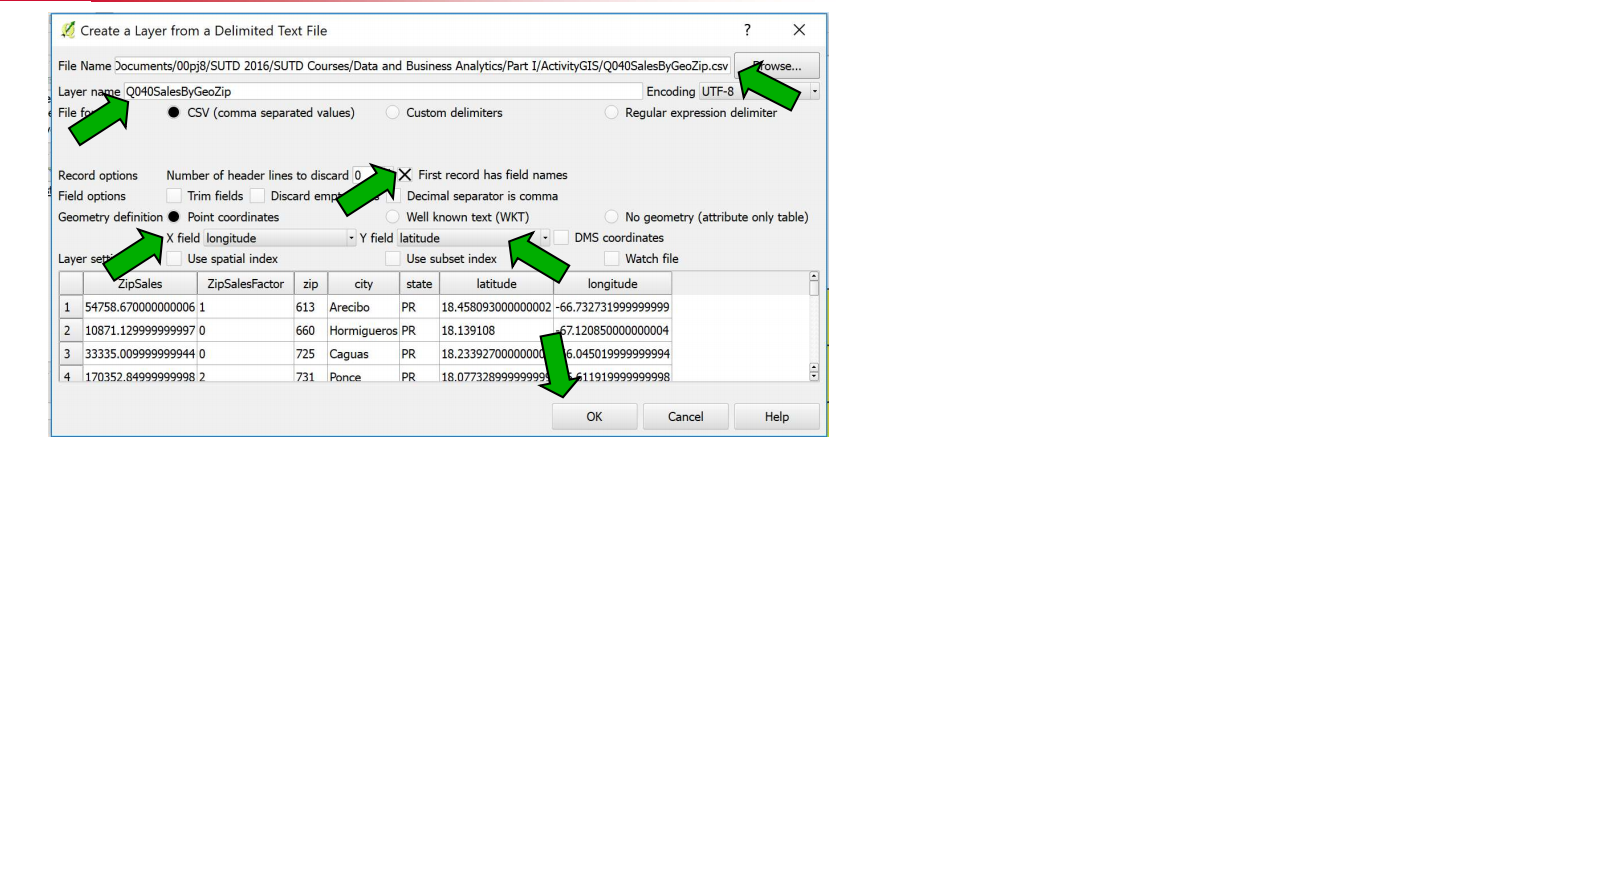
\includegraphics{gis}
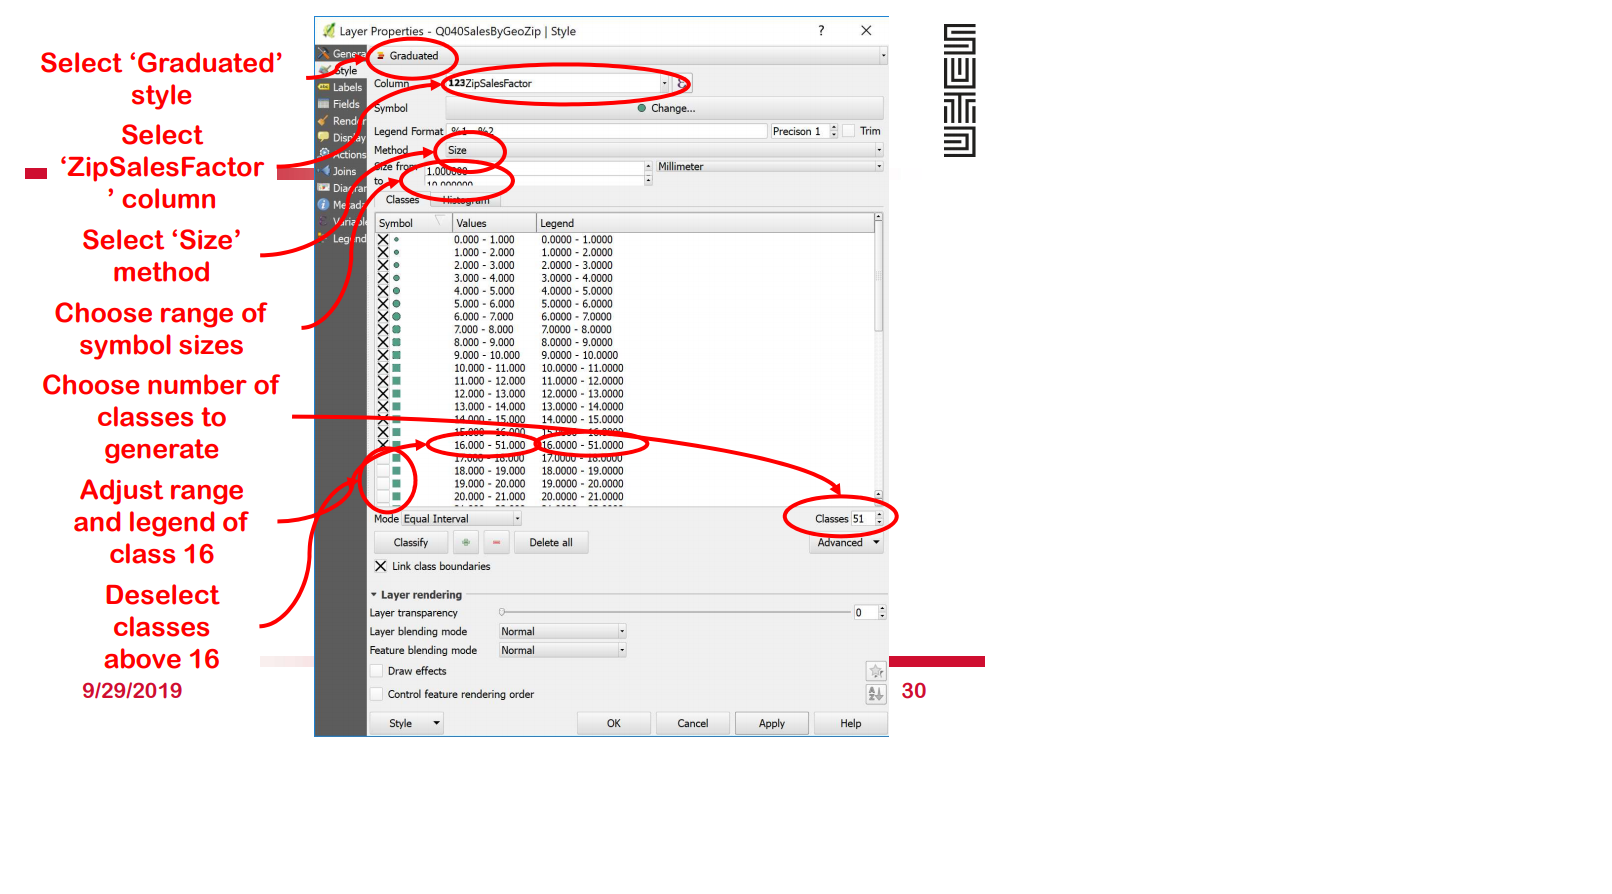
\includegraphics{gis2}
\section{functional modelling}
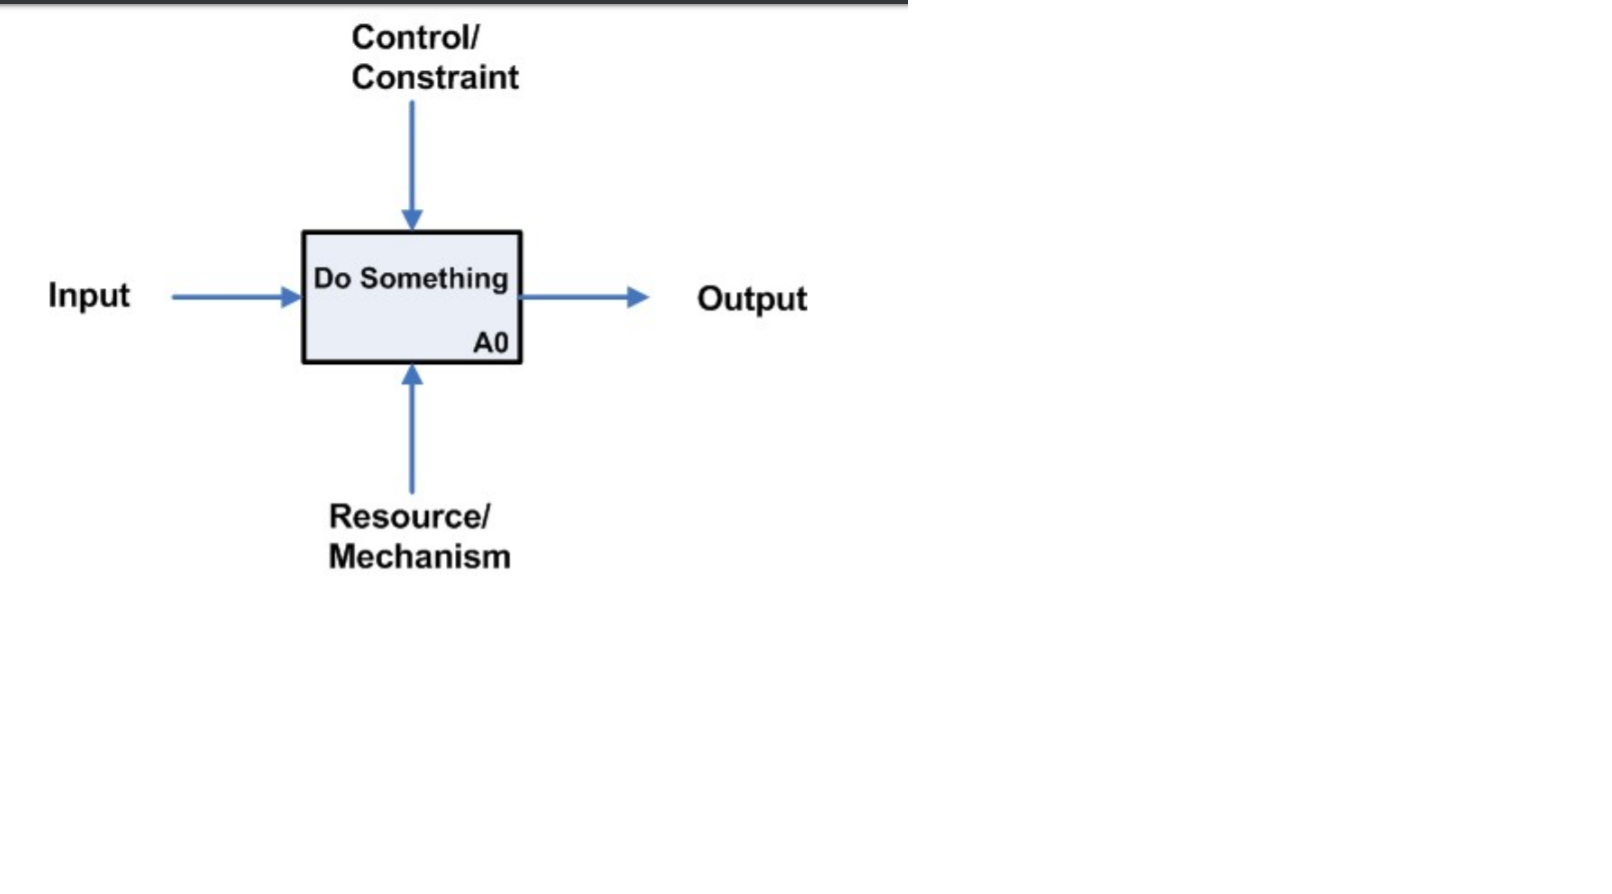
\includegraphics{idef}
\section{Timeseries}
\begin{verbatim}
  hw <- HoltWinters(AirPassengers) #Holt-Winter
  hw <- HoltWinters(AirPassengers,gamma=False) #Holt2
  hw <- HoltWinters(AirPassenger,beta=False, gamma=False)#Holt1
\end{verbatim}
Holt 2 is to capture changing trend like a down curve\\
Holt 1 is to consider newer months more\\
Moving average has no trend, takes evenly from a couple of points.\\
\begin{verbatim}
  tsactuals <- ts(actuals,frequency=12) we need to convert actuals vector to time series specifying frequency to use holt-winters
  hw <- Holtwinters(tsactuals)
  hwfitted <- fitted(hw)[,1]
  #get only first column
  forecasts <- round(as.numeric(fitted(hw)[,1]))

  #calculate WAPE
  actualsnew <- tail(actuals,length(forecasts))
  errors <- forecast-actualsnew
  abserrors <- abs(errors)
  totalerror <- sum(abserrors)
  if (totalactual=0){
  relativeabserror<-totalerror/totalactual
  }else{
  relativeabserror <- 0
  }
  Wape <- relativeabsoerror*100
\end{verbatim}
\section{Credits}
http://www.sqltutorial.org/sql-cheat-sheet/\\
https://www.w3schools.com/sql
\end{document}
